\subsection*{Worse Case of Four Samples}
\\
\\
Similar to the ideal 4 sample test, we consider the following possibilities:

\begin{itemize}
  \item For all the samples negative. The probability is $(1-p)^4$. Only 1 test is required.
  \item For 1 of the samples positive, 3 of the samples negative. The probability is $p(1-p)^3$. 5 tests is required.
  \item For all the samples positive. The probability is $p^4$. 5 tests is required.
  \item For 3 of the samples positive and 1 negative. The probability is $p^3(1-p)$.  5 tests is required.
  \item For 2 of the samples positive, 2 negative. The probability is $p^2(1-p)^2$.  5 tests is required.
  \item For all the samples positive. The probability is $(1-p)^4$. 5 tests is required. 
\end{itemize}
The new expected number of test will be given out by:
\\
\begin{displaymath}
T(p)=5p^{4}+5p^{3}(1-p) \times 4+5 p^{2}(1-p)^{2} \times 6+5p(1-p)^{3} \times 4+1(1-p)^{4}
\end{displaymath}
\\
Simplifying $T(p)$, we get:
\\
\begin{displaymath}
T(p)=-4p^4+16p^3-24p^2+16p+1
\end{displaymath}
\\
For solving $T(p)=3$, we get:
\\
\begin{center}
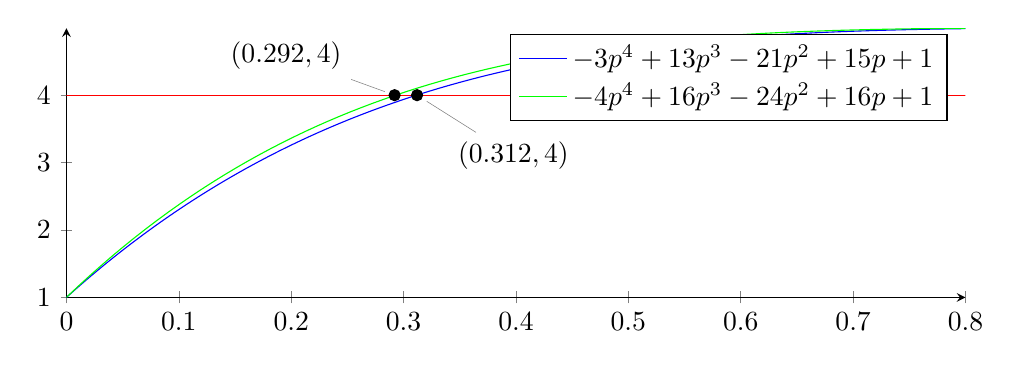
\begin{tikzpicture}
\begin{axis}[
    axis lines = left,
    ytick={1,2,3,4,5},
    xmin=0.0,xmax=0.8,
    xtick={0,0.1,0.2,0.3,0.4,0.5,0.6,0.7,0.8},
    height=5cm,
    width=13cm,
]

\addplot [
    domain=0:1, 
    samples=1000, 
    color=blue,
    ]
    {-3*x^4 + 13*x^3 - 21*x^2 + 15*x + 1};
\addlegendentry{\(-3p^{4}+13p^{3}-21p^{2}+15p+1\)}

\addplot [
    domain=-0:1, 
    samples=100, 
    color=green,
    ]
    {-4*x^4+16*x^3-24*x^2+16*x+1};
\addlegendentry{\(-4p^4+16p^3-24p^2+16p+1\)}

\addplot [
    domain=0:1, 
    samples=100, 
    color=red,
    ]
    {4};

\addplot[mark=*] coordinates {(0.292,4)} node[pin=160:{$(0.292,4)$}]{} ;
\addplot[mark=*] coordinates {(0.312,4)} node[pin=310:{$(0.312,4)$}]{} ;

\end{axis}
\end{tikzpicture}
\end{center}
\\
From the graph, we find that in the worse case, when the group size is equal to 3, pooling should be used only when $p<0.292$ such that the expected amount of tests used is lower than the traditional way. Also, we noticed that the range of  p $(p<)$ is as same as when sample equals to 2.
\\
\\
We can compare the two expected functions by considering the difference:
\\
\begin{displaymath}
D(p)=T(p)-t(p)=-4p^4+16p^3-24p^2+16p+1-(-3p^{4}+13p^{3}-21p^{2}+15p+1)
\end{displaymath}
\\
Solving $D(p):$
\\
\begin{displaymath}
D(p)=-p^4+3p^3-3p^2+p
\end{displaymath}
\\
The difference of the two equations is a quadratic equation.
\\
\\
Graphing the equation:
\\
\begin{center}
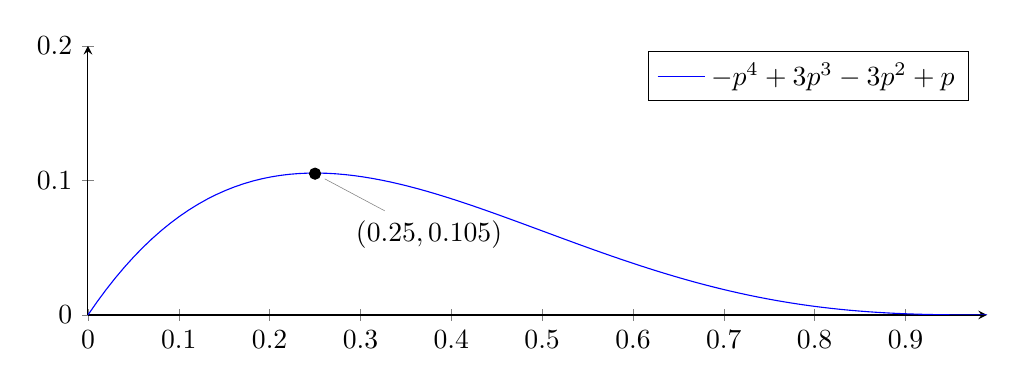
\begin{tikzpicture}
\begin{axis}[
    axis lines = left,
    ytick={0,0.1,0.2},
    ymin=0.0,ymax=0.2,
    xtick={0,0.1,0.2,0.3,0.4,0.5,0.6,0.7,0.8,0.9,1},
    height=5cm,
    width=13cm,
]

%Here the blue parabola is defined
\addplot [
    domain=0:1, 
    samples=100, 
    color=blue,
    ]
    {-x^4 + 3*x^3 -3*x^2 +x};
\addlegendentry{\(-p^4+3p^3-3p^2+p\)}

%Two dots are defined
\addplot[mark=*] coordinates {(0.25,0.105)} node[pin=310:{$(0.25,0.105)$}]{} ;

\end{axis}
\end{tikzpicture}
\end{center}
\\
From the graph, we can see that the vertex of the equation is $(0.25,0.105)$, which means that the biggest difference occurs when $p=0.25$ and the expected value of the two models differ by 0.148 tests.